\chapter{Standalone C++ Analysis framework}
\label{chap:rootframework}

\begin{figure}[htbp]
\centering
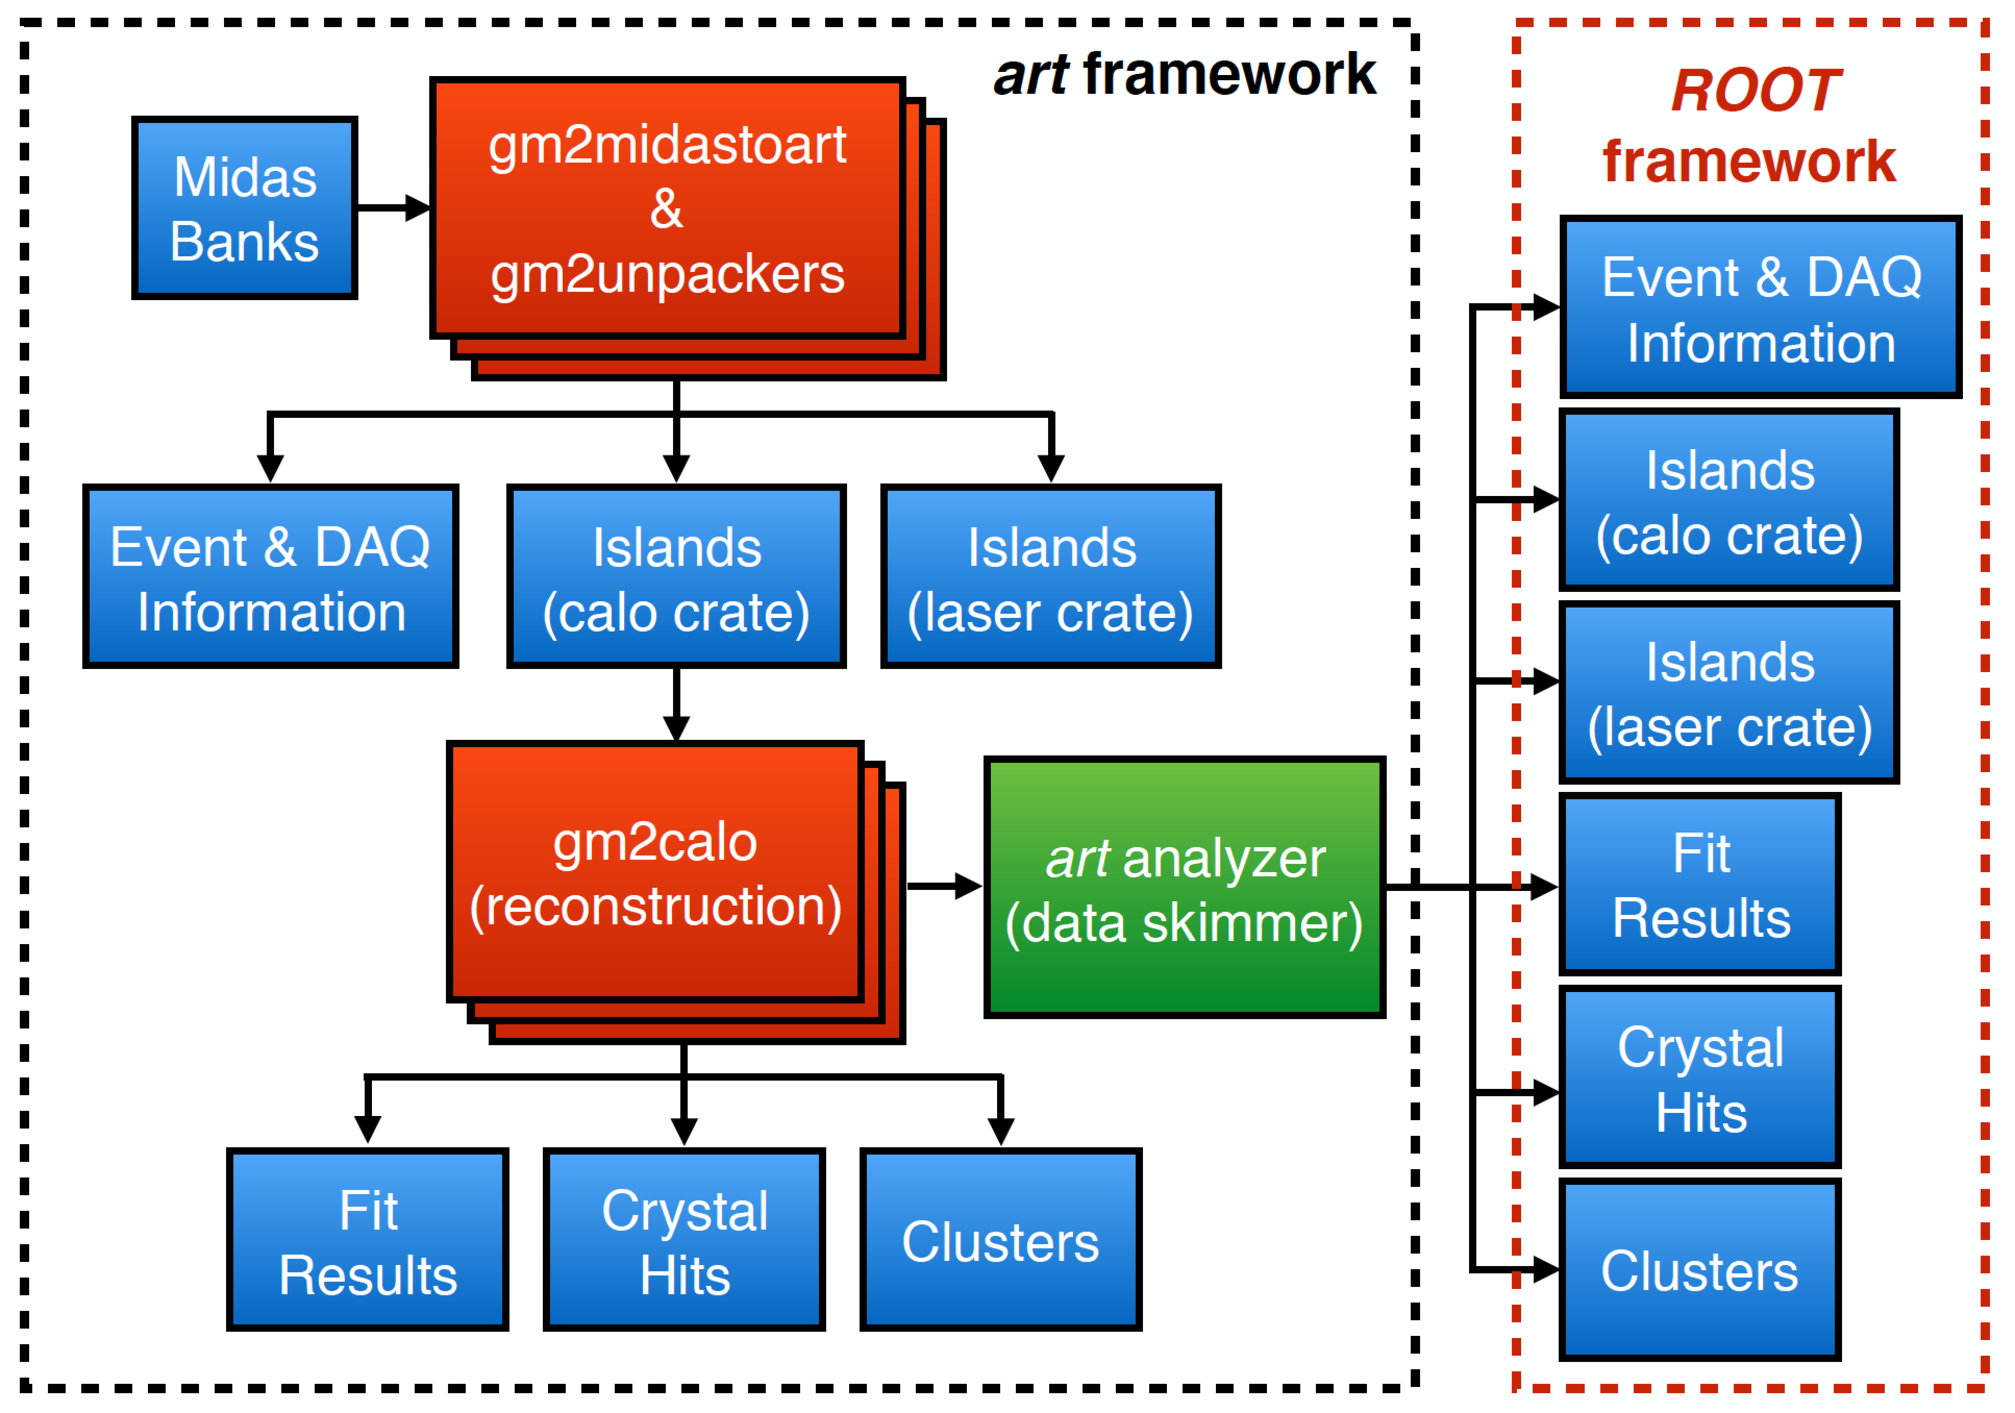
\includegraphics[width=0.7\textwidth]{pics/offline_slac_framework}
\caption{Offline \textit{art} and ROOT framework for the SLAC experimental data.}
\end{figure}

The package \verb+SLAC2016Ana+ contains an example \verb+C+++ framework to help you getting started. You can get it from the github.com by using the following command:
%
\begin{Verbatim}[frame=single]
git clone https://github.com/kimsiang/SLAC2016+. 
\end{Verbatim}
%
You can build your additional analysis code on top of this example or write a new one based on it. The example is already running but it's not doing much yet. You can compile the analysis code by first sourcing your ROOT environment
%
\begin{Verbatim}[frame=single]
source thisroot.sh
\end{Verbatim}
%
and then followed by executing the command
\begin{Verbatim}[frame=single]
make
\end{Verbatim}
%
This will read the necessary ingredients for compilation from the \verb+Makefile+ in the same directory. Don't have to worry much about this file at the moment unless you want to add in more classes to the analysis code.
The point is that it creates an executable named \verb+ana+. You can then execute the program by the command 
%
\begin{Verbatim}[frame=single]
./ana input.script
\end{Verbatim}
%
where \verb+input.script+ includes a path to the root file that you want to analyze (e.g. \verb+./test.root+). 

A description of the individual components of the example are given in the following list. Indicated are also the places where you should start adding your own code:

\begin{itemize}
\item  \verb+main.cxx+: This is the first starting point. It contains the \verb+main()+ function which is necessary for any \verb+C+++ program. The first step is to create instances of \verb+MyAna()+ class which is implemented in the files \verb+MyAna.h+ and \verb+MyAna.C+ (explained in the next items). The \verb+TChain+ represents the ROOT tree discussed in section 3. The files which should be read from disk are specified in the function \verb+Add(filename)+. The tree is then read and processed by the \verb+MyAna()+ class which takes the \verb+TChain+ as argument. The real work is then done in the \verb+Loop()+ function of the \verb+MyAna()+ class which is discussed in the next two items. 

\item \verb+MyAna.h+: Definition of the class \verb+MyAna+, which inherits from the \verb+TTree::MakeClass+. It declares variables and ROOT objects that will be used or stored in your analysis. Several basic functions that are common among event-based particle physics analysis like \verb+initialize()+, \verb+clear()+, \verb+execute()+ and\verb+finalize()+ are declared here.
%% to myself
%% need to change the names like Loop, execute, etc because it is a bit confusing
\item \verb+MyAna.C+: The main function which is called automatically which processing the ROOT trees are \verb+Loop()+. The \verb+Loop()+ function is called only once per run. In the \verb+Loop()+ function, \verb+initialize()+ is called at the beginning of the analysis run, \verb+clear()+ and \verb+execute()+ is called every event, and \verb+finalize()+ at the end of the analysis run.

\item \verb+t1.h+: Header file for the class \verb+t1+ created using \verb+TTree::MakeClass+.  

\item \verb+t1.C+: Source file for the class \verb+t1+ created using \verb+TTree::MakeClass+. The class \verb+Loop()+ is used by \verb+MyAna+ to loop through each \verb+TBranch+.

\item \verb+PlotAll.C+: A ROOT macro which can be used for automatic plotting of a set of histograms which are stored in a ROOT file. Please read the header of the file on how to use it. 
\end{itemize}

\section{Data format and structure for the ROOT tree}

The data samples for this tutorial are stored in ROOT trees. The tree contains a collection of variables (called branches) which are filled once per event (could be 1 or more electrons). The list of variables along with their data type and further explanations are given in the following.

\subsection*{For studies using higher level objects}

\begin{itemize}

\item \verb+FitResult_EventNum+ (\verb+vector<int>+): event number of this fit result
\item \verb+FitResult_CaloNum+ (\verb+vector<int>+): calorimeter number of this fit result
\item \verb+FitResult_XtalNum+ (\verb+vector<int>+): crystal number of this fit result
\item \verb+FitResult_IslandNum+ (\verb+vector<int>+): island number of this fit result
\item \verb+FitResult_UtcaSlotNum+ (\verb+vector<int>+): utca slot number of this fit result
\item \verb+FitResult_ChannelNum+ (\verb+vector<int>+): rider channel number of this fit result
\item \verb+FitResult_Energy+ (\verb+vector<double>+): energy (number of photons) of this fit result
\item \verb+FitResult_Time+ (\verb+vector<double>+): time (clock tick of 800 MHz) of this fit result within the fill/event
\item \verb+FitResult_Pedestal+ (\verb+vector<double>+): pedestal of this fit result
\item \verb+FitResult_Chi2+ (\verb+vector<double>+): Chi squared of this fit result
\item \verb+FitResult_ClockCounter+ (\verb+vector<long long>+): time stamp (clock tick of 40 MHz) of this fit result from Rider header information

\item \verb+XtalHit_EventNum+ (\verb+vector<int>+): event number of this crystal hit
\item \verb+XtalHit_CaloNum+ (\verb+vector<int>+): calorimeter number of this crystal hit
\item \verb+XtalHit_XtalNum+ (\verb+vector<int>+): crystal number of this crystal hit
\item \verb+XtalHit_IslandNum+ (\verb+vector<int>+): island number of this crystal hit
\item \verb+XtalHit_UtcaSlotNum+ (\verb+vector<int>+): utca slot number of this crystal hit
\item \verb+XtalHit_ChannelNum+ (\verb+vector<int>+): rider channel number of this crystal hit
\item \verb+XtalHit_Energy+ (\verb+vector<double>+): energy (number of photons) of this crystal hit
\item \verb+XtalHit_Time+ (\verb+vector<double>+): time (clock tick of 800 MHz) of this crystal hit within the fill/event
\item \verb+XtalHit_ClockCounter+ (\verb+vector<long long>+): time stamp (clock tick of 40 MHz) of this crystal hit from Rider header information

\item \verb+Cluster_EventNum+ (\verb+vector<int>+): event number of this cluster 
\item \verb+Cluster_CaloNum+ (\verb+vector<int>+): calorimeter number of this cluster
\item \verb+Cluster_IslandNum+ (\verb+vector<int>+): island number of this cluster
\item \verb+Cluster_Energy+ (\verb+vector<double>+): energy (number of photons) of this cluster
\item \verb+Cluster_Time+ (\verb+vector<double>+): time (clock tick) of this cluster 
\item \verb+Cluster_X+ (\verb+vector<double>+): local x-position of this cluster (logarithmic-weighted)
\item \verb+Cluster_Y+ (\verb+vector<double>+): local x-position of this cluster (logarithmic-weighted)

\item \verb+Italiano_EventNum+ (\verb+vector<int>+): event number of this analyzed laser crate waveform
\item \verb+Italiano_CaloNum+ (\verb+vector<int>+): calorimeter number of this analyzed laser crate waveform
\item \verb+Italiano_XtalNum+ (\verb+vector<int>+): crystal number of this analyzed laser crate waveform
\item \verb+Italiano_IslandNum+ (\verb+vector<int>+): island number of this analyzed laser crate waveform
\item \verb+Italiano_UtcaSlotNum+ (\verb+vector<int>+): utca slot number of this analyzed laser crate waveform
\item \verb+Italiano_ChannelNum+ (\verb+vector<int>+): rider channel number of this analyzed laser crate waveform
\item \verb+Italiano_Amplitude+ (\verb+vector<double>+): amplitude (ADC samples) of this analyzed laser crate waveform
\item \verb+Italiano_Time+ (\verb+vector<double>+): time (clock tick of 800 MHz) of this analyzed laser crate waveform within the fill/event
\item \verb+Italiano_Pedestal+ (\verb+vector<double>+): pedestal of this analyzed laser crate waveform
\item \verb+Italiano_Area+ (\verb+vector<double>+): Area of this analyzed laser crate waveform
\item \verb+Italiano_ClockCounter+ (\verb+vector<long long>+): time stamp (clock tick of 40 MHz) of this analyzed laser crate waveform from Rider header information
\end{itemize}

\subsection*{For studies using lower level objects}
Blow are the Tleaves of the \verb+islandTree+.

\begin{itemize}
\item \verb+RunNum+ (\verb+int+): run number of this island
\item \verb+EventNum+ (\verb+int+): event number of this island
\item \verb+FillType+ (\verb+int+): fill type of this island (1 is muon fill, 2 is laser fill)
\item \verb+TriggerNum+ (\verb+int+): trigger number of this island
\item \verb+CaloNum+ (\verb+int+): calorimeter number of this island
\item \verb+XtalNum+ (\verb+int+): crystal number of this island
\item \verb+IslandNum+ (\verb+int+): island number of this island
\item \verb+UtcaSlotNum+ (\verb+int+): utca slot number of this island
\item \verb+ChannelNum+ (\verb+int+): rider channel number of this island
\item \verb+Length+ (\verb+int+): number of sample of this island
\item \verb+Time+ (\verb+int+): time (clock tick of 800 MHz) of the first sample of this island within the fill/event
\item \verb+ClockCounter+ (\verb+long+): time stamp (clock tick of 40 MHz) of this island from Rider header information
\item \verb+Trace+ (\verb+vector<short>+): ADC samples of this island
\end{itemize}

